\documentclass[../main.tex]{subfiles}
\graphicspath{{../figures/}}
\usepackage[linesnumbered,ruled,vlined,resetcount,algochapter]{algorithm2e}

\begin{document}

\mychapter{面向少样本提示学习模型的双重对比知识蒸馏方法}
\label{sec:ch3-dual-contrastive-distillation-for-few-shot-prompts}

\mysection{引言}
\label{sec:ch3-1-introduction}

在深度模型构建以数据/知识层为根基。该层为模型提供了理解与泛化所需的信息基础,其质量与可复用性直接决定了下游建模与搜索的起点与上限。然而,现实场景中高质量标注数据的稀缺性与任务间的分布差异构成了核心瓶颈,单纯扩充数据或端到端再训练往往代价高昂、收益递减。鉴于此,本章聚焦于数据/知识层的迁移优化,旨在探索以知识换数据的复用路径。为此,本章提出 Prompt-Distiller 方法,通过可控提示与双教师协同蒸馏,将不同来源模型中沉淀的任务相关知识以更高的样本效率转移到目标表示中。其核心思想是以迁移为轴,将外部先验与弱标注信号转化为对目标表征的约束与指导,从而在有限标注下获得对任务结构更敏感、更可搜索的表示,为后续的神经架构构建提供更低的试错成本与更稳定的起步性能。

在大规模预训练语言模型(Pre-trained Language Model,PLM)取得突破性进展后,深度模型的高效构建成为自然语言处理领域的重要研究方向之一。预训练-微调范式\cite{bertpretraining_devlin_2019}通过在海量无标注语料上预训练模型参数,然后在下游任务上进行监督微调,实现了对下游任务的显著性能提升。然而,传统微调方法通常要求下游任务有足够大的人工标注数据集支撑模型训练,这在实际应用中往往难以满足,限制了PLM的适用范围。为了解决小样本场景下模型难以训练的问题,提示学习方法应运而生。提示学习通过构造任务相关的提示,将下游任务统一转换为完形填空形式,使模型利用预训练时储存的知识直接预测答案。例如,Schick 等人提出的 PET 方法\cite{exploitingclozequestions_schick_2021}使用了手工设计的提示模板,将情感分类任务转化为填空句“这部电影非常[MASK]”,由模型预测被遮蔽位置的词语,从而判断情感极性。这类方法有效地缩小了预训练任务与下游任务之间的差距,在极少标注数据的条件下显著提高了模型性能。特别地,随着模型规模的增加,PLM 所蕴含的知识更加丰富,提示学习在小样本、甚至零样本任务上表现出更强的效果。例如,GPT-3、ERNIE 3.0 和 FLAN 等超大规模模型在完全零样本的情形下即可在多个NLP任务上取得接近有监督训练的效果\cite{languagemodelsare_brown_2020,ernie3.0large_sun_2021,finetunedlanguagemodels_wei_2022}。然而,大规模模型(参数量往往达到数亿甚至百亿)在推理部署时的计算和存储开销极其高昂,难以直接应用于资源受限的在线系统中。如何在保持模型性能的前提下压缩PLM规模,从而实现深度模型的高效部署,已成为一个亟待解决的问题。

知识蒸馏(Knowledge Distillation,KD)提供了一种有前景的模型压缩方案。KD 采用“教师模型-学生模型”的学习架构:通过让一个规模较大的预训练教师模型指导一个小规模学生模型的训练,将教师模型中蕴含的知识蒸馏到学生模型中。相比直接训练小模型,知识蒸馏往往能获得更优的性能,因为教师模型的输出提供了关于任务的软知识(即类间的概率分布信息,亦称暗知识)以及模型内部的特征表示等提示信息。近年来,针对BERT等预训练模型的蒸馏研究大量涌现。例如, Hinton 等人提出的 Vanilla KD 方法\cite{distillingknowledgeneural_hinton_2015}仅利用教师模型输出的对数几率作为软目标来训练学生模型;Sun 等人提出的 Patient KD\cite{patientknowledgedistillation_sun_2019}进一步利用教师模型若干中间层的隐藏表示向量指导学生模型对应层的训练,以逐层逼近教师的特征表示;Jiao等人的TinyBERT方法\cite{tinybertdistillingbert_jiao_2020}则结合上述思想,设计了包含输出层logits、词嵌入层表示及中间层自注意力矩阵等多方面的知识蒸馏损失,大幅提升了蒸馏效果。然而,上述知识蒸馏技术主要面向传统的微调范式,即教师模型采用任务特定的分类头进行监督训练。在这种情况下,有充足的标注数据可用于蒸馏训练,且教师模型输出的logits直接对应预定义的类别。然而,针对提示学习范式下的模型压缩问题,上述技术并不能直接套用。首先,提示学习中教师模型通常通过在 [MASK] 位置预测标签词来完成分类任务,其输出空间与原预训练任务(如遮掩语言模型)相同而非固定类别数,这与传统KD的输出形式存在差异。其次,更具挑战性的是,小样本提示学习场景中标注数据极其匮乏,仅靠少量监督信号难以充分指导学生模型训练,甚至会导致学生模型严重过拟合教师模型而失去泛化能力。换言之,在仅有 $N\times K$($N$ 类,每类 $K$ 个样本)监督样本的条件下,让学生模型去学习一个庞大教师模型的全部知识,任务颇为艰巨。以上挑战引出了一个核心问题:在少样本提示学习场景下,如何有效地将一个提示微调的PLM教师模型蒸馏到小规模学生模型上?

为了解决上述问题,本章提出了一种 Prompt-Distiller 算法,用于在少样本场景下对提示微调的PLM进行知识蒸馏,从而构建高效小模型部署方案。本章方法的核心思想在于:引入双教师学习机制与基于对比学习的中间层知识对齐,以最大程度缓解小样本条件下学生模型过拟合和知识缺失的问题。具体而言,我们让学生模型同时从两个教师模型中学习知识:一个是针对下游任务经过提示微调的教师模型,提供任务特定知识指导;另一个是教师模型在下游任务微调前的原始预训练模型,提供通用预训练知识辅助。在蒸馏训练时,学生模型不仅要拟合提示微调教师模型在标注样本上的输出分布,还通过无监督数据学习原始预训练教师的输出分布,从而将大量通用语言知识融入学生模型中。这种双教师方案有助于弥补标注数据匮乏导致的知识盲区。此外,针对教师与学生模型容量相差悬殊、直接对齐中间层表示效果不佳的问题,本章设计了一种探针对比蒸馏策略。我们为教师模型和学生模型的各层隐藏状态分别训练轻量级的MLM探针分类器,用于预测下游任务的标签词分布。然后,通过构造正负样本对比,我们引导学生模型的各层探针输出与教师模型对应层的探针输出保持相似的分布差异(即学习高阶依赖关系),而非简单逐点匹配隐藏向量。通过这种对比学习技巧,我们在一定程度上规避了大模型与小模型直接匹配带来的不适配问题,进一步提升了蒸馏效果。

本章余下部分组织如下:首先在第 \ref{sec:ch3-2-problem-definition} 节明确本章所解决的问题及相关场景设定,给出形式化定义;第 \ref{sec:ch3-3-prompt-distiller-framework} 节详细阐述Prompt-Distiller算法的理论框架与模型设计,包括双教师蒸馏和基于对比学习的中间层知识转移机制,并以公式推导方式给出各部分损失函数及整体优化目标;随后在第 \ref{sec:ch3-4-prompt-distiller-implementation} 节给出算法的实现细节与伪代码描述;第 \ref{sec:ch3-5-experiments-and-analysis} 节设计了广泛的对比实验与消融分析,验证本章方法在多个少样本任务上的有效性;最后第 \ref{sec:ch3-6-chapter-summary} 节对本章工作进行总结,并说明本章研究结果对于后续章节系统实现的支撑作用。通过本章的研究,将为下一章的小模型部署系统实现提供坚实的理论和方法基础。

\mysection{问题定义}
\label{sec:ch3-2-problem-definition}
本章探讨少样本提示学习模型的知识蒸馏问题。场景设定如下:假定存在一个规模庞大的预训练语言模型作为教师模型$\Theta_T$,其经过少量标注数据的提示微调后能够在目标任务上取得较高性能;同时希望训练一个参数规模更小的学生模型$\Theta_S$,使其在该任务上的性能接近教师模型但推理效率更高。为了限定问题范围,我们考虑典型的$N$-分类任务(例如情感分类、自然语言推理等)。少样本设定下,训练集中每一类别仅有$K$个标注样本,整个训练集记为$X={(x_i, y_i)}$,其中$x_i$表示第$i$个输入文本,$y_i \in \mathcal{Y}$为其对应的类别标签,$\mathcal{Y}$为标签集合且$|\mathcal{Y}| = N$。因此,标注训练集规模仅为$N \times K$。通常$K$很小,例如$K=16$或$32$(典型few-shot设置)。此外,我们假定还可获取一定量的无标注语料$\tilde{X}={x_j'}$,其规模约为标注集的$n$倍(即$|\tilde{X}| = n\cdot |X|$),这些语料与任务领域大致相关但未经过人工标注。无标注数据可用于辅助蒸馏训练,为学生模型提供额外的自监督信号。需要强调的是,本章方法并不依赖$\tilde{X}$的具体内容或来源,它可以来自于任务相关的公开数据或在线爬取的文本。

在模型训练流程上,教师模型$\Theta_T$首先通过提示微调在少样本集$X$上进行训练,使其适应目标任务。本章采用 PET 方法\cite{exploitingclozequestions_schick_2021} 作为提示微调手段,即利用若干人工设计的提示模板将原始输入$x$转换为带有 [MASK] 占位符的提示输入,然后引导模型在遮蔽位置预测一个预先定义的标签词 $l(y)$ 作为分类结果。例如,对于情感分类任务,标签集合 $\mathcal{Y}$ 以及可选用的标签词集合可能为:
\begin{gather}
	\mathcal{Y}=\{\text{正面}, \text{负面}\} \\
	l(\text{正面})=\text{“great”},\quad l(\text{负面})=\text{“terrible”}
\end{gather}
通过在样本$x_i$对应的提示模板中填入 [MASK],让 PLM 预测该位置上的输出词语,即可完成分类。我们用$s_{\Theta}(l(y)\mid x_i)$表示模型$\Theta$在输入$x_i$(经提示包装后)条件下,输出词为标签词$l(y)$的打分。教师模型$\Theta_T$在提示微调完成后,其在任务上的预测概率定义如下:对于任意输入文本$x_i$和类别$y\in\mathcal{Y}$,教师模型预测$x_i$属于类别$y$的概率为:
\begin{equation}
	\label{eq:teacher-prob}
	p_{T}(y \mid x_i) = \frac{\exp\big(s_{\Theta_T}(l(y)\mid x_i)\big)}{\displaystyle\sum_{y' \in \mathcal{Y}} \exp\big(s_{\Theta_T}(l(y')\mid x_i)\big)} .
\end{equation}
其中$\exp(\cdot)$表示指数函数,分母部分遍历$\mathcal{Y}$中所有可能类别对应的标签词。\eqref{eq:teacher-prob} 与 Softmax 函数形式一致,表示教师模型$\Theta_T$在看到输入$x_i$时,输出属于类别$y$的相对概率。与传统微调的分类头不同,这里的概率分布是通过MLM头在词汇表上针对标签词计算得到的。利用这样的概率输出,可以进一步定义教师模型在$x_i$上的交叉熵损失或其他指标。本章后续将主要利用$p_T(y\mid x_i)$作为教师模型输出的软标签指导学生模型的训练。

为衡量学生模型的性能,我们需要定义学生模型$\Theta_S$的预测输出形式。类似地,在提示模板下,学生模型预测$x_i$属于类别$y$的概率可表示为:
\begin{equation}
	\label{eq:student-prob}
	p_{S}(y \mid x_i) = \frac{\exp\big(s_{\Theta_S}(l(y)\mid x_i)\big)}{\displaystyle\sum_{y' \in \mathcal{Y}} \exp\big(s_{\Theta_S}(l(y')\mid x_i)\big)} .
\end{equation}

有了上述定义,我们可以进一步刻画知识蒸馏的目标:希望通过训练使得对于任意输入$x_i$,学生模型的输出分布$p_S(\cdot \mid x_i)$尽可能贴近教师模型的输出分布$p_T(\cdot \mid x_i)$,同时学生模型也正确地拟合样本的真实标签。在少样本条件下,实现这一目标需要克服教师-学生容量差距大、训练样本少导致的过拟合等难题。

为便于描述,表\ref{tab:ch3-notation}汇总了本章涉及的主要符号及意义。可以看到,我们区分了两种教师模型:$\Theta_T$表示提示微调后的教师模型,而$\Theta_{T'}$则表示提示微调前的教师模型(即原始预训练模型)。$\Theta_{T'}$和$\Theta_T$在结构上相同,但前者未经下游任务微调,后者则在数据$X$上进行了提示学习训练。由于提示学习并未改变模型的结构和参数规模,因此$\Theta_{T'}$可看作$\Theta_T$的初始化或原型。正如引言所述,我们将$\Theta_T$和$\Theta_{T'}$都视为教师,在不同环节为学生模型提供知识。需要指出的是,$\Theta_{T'}$不是通过其他数据训练而来,而是$\Theta_T$在进行提示微调之前的原始状态;也就是说,$\Theta_{T'}$已经过海量预训练语料的学习,蕴含广泛的通用语言知识,只是尚未针对特定下游任务调整。

\begin{table}[htbp]
	\centering
	\bicaption[本章符号说明]{本章主要符号及说明}[Chapter notation]{Major symbols and descriptions used in this chapter}
	\label{tab:ch3-notation}
	\small\begin{tabular}{ll}
		\toprule[1pt]
		符号                       & 含义                                                       \\
		\midrule[0.5pt]
		$\mathcal{Y}$            & 下游任务的标签集合,$|\mathcal{Y}|=N$。                             \\
		$X = \{(x_i, y_i)\}$     & 少样本标注训练集,每类$K$个样本,总计$N \times K$条。                       \\
		$\tilde{X} = \{x_j'\}$   & 无标注辅助训练集,规模$|\tilde{X}| = n \cdot |X|$。                  \\
		$l(y)$                   & 标签$y$对应的标签词,在提示模板中填入[MASK]进行预测。                          \\
		$\Theta_T$               & 提示微调后的教师模型参数(大模型)。                                       \\
		$\Theta_{T'}$            & 提示微调前的教师模型参数(大模型,$\Theta_T$的原始预训练状态)。                    \\
		$\Theta_S$               & 学生模型参数(小模型)。                                             \\
		$s_{\Theta}(l(y)\mid x)$ & 模型$\Theta$对输入$x$输出类别$y$对应标签词$l(y)$的打分。                   \\
		$p_T(y\mid x)$           & 教师模型$\Theta_T$预测$x$属于类别$y$的概率,公式\eqref{eq:teacher-prob}。 \\
		$p_S(y\mid x)$           & 学生模型$\Theta_S$预测$x$属于类别$y$的概率,公式\eqref{eq:student-prob}。 \\
		$N_T, N_S$               & 教师模型和学生模型的Transformer编码层数(不含输出层)。                        \\
		$P_T^{(j)}, P_S^{(k)}$   & 教师第$j$层、学生第$k$层隐藏表示对应的探针分类器。                             \\
		\bottomrule[1pt]
	\end{tabular}
\end{table}

基于以上符号定义,我们将少样本提示学习情境下的知识蒸馏问题形式化为:在给定$\Theta_T$和少量$X$的前提下,如何利用$X$及$\tilde{X}$训练得到学生模型参数$\Theta_S^*$,使得$\Theta_S^*$在验证/测试集上的预测性能尽可能接近$\Theta_T$。需要确保$\Theta_S^*$的参数规模远小于$\Theta_T$,以实现模型压缩和高效部署。本章后续部分将围绕该问题展开,提出具体的模型蒸馏策略和优化方法。

\mysection{Prompt-Distiller算法框架}
\label{sec:ch3-3-prompt-distiller-framework}
针对上述问题定义,本节提出Prompt-Distiller算法的总体框架和原理。如图\ref{fig:PromptDistillerFramework}所示,Prompt-Distiller包含两个核心模块:其一是来自双教师模型的监督知识蒸馏,即学生模型同时从提示微调教师$\Theta_T$和原始预训练教师$\Theta_{T'}$两方面获取知识信号;其二是基于探针的对比学习式中间层知识转移,即通过比较教师与学生模型中间表示对下游任务的输出差异,促进学生学习教师模型更深层次的判别能力。下面分别对这两个模块展开论述。

\begin{figure}[htbp]
	\centering
	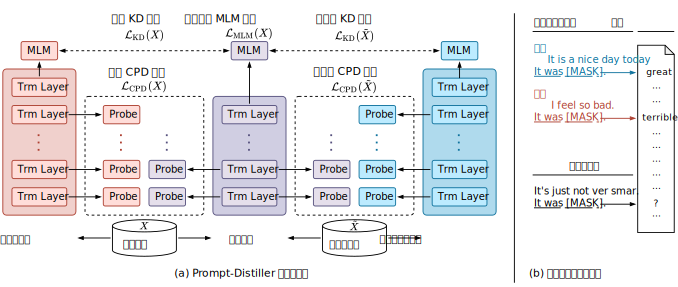
\includegraphics[width=0.95\textwidth]{Prompt-Distiller/framework.pdf}
	\bicaption{(a) Prompt-Distiller 框架示意图。学生模型在提示微调教师模型(左)与原始预训练教师模型(右)的联合指导下进行训练:一方面蒸馏二者在输出层的预测分布,另一方面通过探针分类器对比中间层表示差异,实现对比学习。(b) 提示增强数据示例,下划线部分表示提示模板中的输入与标签词片段。}{(a) Schematic illustration of the Prompt-Distiller framework. The student model is trained under the joint guidance of a prompt-tuned teacher and the original pretrained teacher: (i) output-level distillation of their prediction distributions, and contrastive learning via probe classifiers that compare intermediate-layer representations. (b) Example of prompt-augmented data, where underlined segments indicate input and label tokens within the prompt template.}
	\label{fig:PromptDistillerFramework}
\end{figure}

\mysubsection{双教师知识蒸馏策略}
\label{sec:ch3-3-1-dual-teacher-distillation-strategy}
1)从提示微调教师获取任务特定知识。 提示微调后的教师模型$\Theta_T$在少样本任务上性能较高,反映了与任务密切相关的知识和模式。为了使学生模型学习这一任务特定知识,我们首先考虑最常用的基于输出层概率分布对齐的蒸馏方法。具体来说,对于每一个标注训练样本$(x_i, y_i) \in X$,令$\vec{y}_i \in {0,1}^N$表示$y_i$对应的独热标签向量,维度为$N$(即正确类别位置为1,其余为0)。学生模型在$x_i$上的预测分布由公式\eqref{eq:student-prob}给出,表示为向量形式$p_S(y\mid x_i)$。将该分布与$\vec{y}_i$计算交叉熵可得学生模型的监督分类损失:
\begin{equation}
	\label{eq:mlm-loss}
	\mathcal{L}_{\text{MLM}}(X) = -\frac{1}{|X|} \sum_{(x_i, y_i)\in X} \sum_{y \in \mathcal{Y}} \vec{y}_i(y)\log p_S(y \mid x_i) .
\end{equation}
其中$\vec{y}_i(y)$表示独热向量在类别$y$对应位置的取值。需要注意的是,这里的MLM指代模型基于遮掩语言模型头进行预测输出。公式\eqref{eq:mlm-loss}即为常规的交叉熵分类损失,保证学生模型能正确拟合少量训练样本的真实标签。

在此基础上,我们引入提示微调教师模型$\Theta_T$输出的软标签信息,作为蒸馏学习的补充监督信号。教师模型$\Theta_T$对于样本$x_i$输出的概率分布已由公式\eqref{eq:teacher-prob}定义为$p_T(y\mid x_i)$,它代表了教师模型对各类别的信心。虽然$x_i$只有一个真实标签,但$p_T(y\mid x_i)$刻画了各类别之间的相对分布,蕴含了教师模型对错误类别的认知和区分能力,即所谓暗知识。蒸馏的思想是希望学生模型也能掌握这种精细的区分模式,而不仅仅是输出正确类别。因此,我们可以让学生模型的输出$p_S(y\mid x_i)$去拟合教师模型的输出分布$p_T(y\mid x_i)$。这可以通过计算两个概率分布之间的交叉熵来实现,即定义有监督蒸馏损失为:
\begin{equation}
	\label{eq:kd-loss-supervised}
	\mathcal{L}_{\text{KD}}(X) = -\frac{1}{|X|}\sum_{(x_i, y_i)\in X} \sum_{y \in \mathcal{Y}} p_T(y \mid x_i) \log p_S(y \mid x_i) .
\end{equation}

上述损失会促使学生模型的输出尽量接近教师模型,在标注样本上保持与教师一致的行为。需要说明的是,有时引入温度系数$\alpha$可使教师输出分布更平滑,从而更好地指导学生。做法是将教师输出的Softmax温度调高,使其概率更接近于均匀分布,然后再用于蒸馏。公式上相当于将$p_T(y\mid x_i)$取$\text{Softmax}(z/\alpha)$,其中$z$为未归一化的logit向量,$\alpha > 1$时产生平滑作用。在本章实验中,我们将根据验证集表现选取适当的温度系数,但公式推导中暂不显式表示$\alpha$。

2)从预训练教师获取通用知识。 虽然提示微调教师提供了宝贵的任务特定知识,但由于少样本学习的限制,其本身可能存在一定的过拟合风险:模型可能记忆了少量训练样本的特点而未能学到一般性规律。特别地,如果$K$极小,教师模型输出的分布$p_T(y\mid x)$在训练样本上可能过于自信(趋近于独热),从而为学生提供的暗知识有限。此外,学生模型参数容量远小于教师模型,很难仅凭少量样本就捕获到教师模型蕴含的大量背景知识。因此,我们考虑利用教师模型在未经过微调时所具有的通用预训练知识来辅助蒸馏。直观上,原始预训练的教师模型$\Theta_{T'}$在大规模语料上已经学习到广泛的语言表达和常识知识,尽管未针对当前任务,但其对语言现象的理解对学生模型仍然是极为有价值的参考。

具体做法是:让学生模型在无标注数据$\tilde{X}$上去拟合预训练教师$\Theta_{T'}$的输出分布。这类似于\emph{蒸馏预训练知识},因为$\Theta_{T'}$的输出反映了模型的预训练记忆,如词汇共现、句法语义等信息。对于每一个无标注样本$x_j' \in \tilde{X}$,我们通过教师模型$\Theta_{T'}$计算其输出分布$p_{T'}(y\mid x_j')$,其中$l(y)$仍沿用下游任务定义的标签词(此时$\Theta_{T'}$实际上是在零样本条件下对任务进行推断)。虽然$x_j'$没有人工标签,但$\Theta_{T'}$可以给出其属于各类别的一个猜测概率分布。我们希望学生模型也能给出类似的分布,从而习得$\Theta_{T'}$在预训练中积累的知识。因此,定义无监督蒸馏损失为:
\begin{equation}
	\label{eq:kd-loss-unsupervised}
	\mathcal{L}_{\text{KD}}(\tilde{X}) = -\frac{1}{|\tilde{X}|}\sum_{x_j' \in \tilde{X}} \sum_{y \in \mathcal{Y}} p_{T'}(y \mid x_j') \log p_S(y \mid x_j') .
\end{equation}

该损失通过无监督数据让学生模仿预训练教师的行为,不需要任何人工标注。尤其在$|\tilde{X}|$远大于$|X|$的情况下,学生模型能够接触更多样的语言现象,缓解了仅凭少数样本学习导致的过拟合。同时,由于$\tilde{X}$覆盖了多样的内容,学生模型通过$\mathcal{L}_{\text{KD}}(\tilde{X})$可学习到更通用的特征表示和对输入的鲁棒理解,这将有助于其提升对未见样本的泛化性能。需要注意的是,在计算$p_{T'}(y \mid x_j')$时,$\Theta_{T'}$仍然采用与$\Theta_T$相同的提示模板和标签词来进行预测,尽管它未经微调,其输出可以被视为对下游任务的零样本预测。这种利用预训练模型进行辅助监督的思想,与自蒸馏或“born-again network”等概念有一定相似之处,但区别在于这里$\Theta_{T'}$并非学生模型的历史版本,而是教师模型本身在未调优时的形态。两种教师模型提供的互补知识可以从不同侧面提升学生模型。

\mysubsection{基于对比学习的中间层知识转移}
\label{sec:ch3-3-2-contrastive-middle-layer-transfer}
上述双教师蒸馏策略主要在输出层利用概率分布提供指导。事实上,深度模型内部各层的中间表示也包含丰富的知识,是知识蒸馏的重要来源。例如,教师模型隐藏层中的特征向量承载了对输入文本在不同抽象级别上的表示,直接对齐这些表示可以让学生模型受益。然而,在我们的场景下,教师为大型模型而学生为小型模型,二者的表示空间和容量相差悬殊。如果强行最小化对应层隐藏向量之间的欧氏距离,可能会由于小模型的表示能力不足而适得其反,甚至拖累训练过程。为此,我们没有选择直接对齐隐藏层向量,而是采用一种探针方法来间接比较教师和学生模型的中间层知识。在训练开始前,我们冻结教师模型$\Theta_T$和学生模型$\Theta_S$当前的参数(学生模型此时尚未训练),为它们各自的每一层隐藏状态训练一个轻量的MLM分类器,即探针,来预测下游任务的标签。这类似于在不同层上探测模型对任务的判别能力。具体而言,对于教师模型的每一个Transformer编码层$j$($j=1,2,\dots,N_T-1$,不含最后输出层),我们训练一个探针分类器$P_T^{(j)}$,它接收该层输出的隐藏表示(通常指[MASK]位置对应的向量)作为输入,输出一个$N$维向量,经过Softmax转化为对$N$个类别的概率分布。训练时,使用少样本集$X$,将探针$P_T^{(j)}$的输出概率与真实标签$\vec{y}_i$计算交叉熵,调整探针参数使其能够利用第$j$层隐藏状态来预测正确类别\footnote{为了保证探针训练的可靠性,可对$X$进行$k$折交叉验证训练探针,以免过拟合。由于$X$极小,此处探针训练只作为蒸馏的辅助步骤,不会引入明显的过拟合。实际应用中也可使用少量额外标注数据训练探针,此处从简处理。}。经过此过程,我们可以得到教师模型从第1层到第$N_T-1$层的一组探针${P_T^{(1)}, P_T^{(2)}, \dots, P_T^{(N_T-1)}}$。同理,为学生模型$\Theta_S$的每一编码层$k$($k=1,2,\dots,N_S-1$)训练探针$P_S^{(k)}$。由于学生模型层数与教师不同,我们不强调层与层的严格对应关系,而是利用所有探针的综合判别能力来设计中间层知识转移策略。

当探针训练完成后,教师模型第$j$层探针$P_T^{(j)}$即可作为观察该层知识的窗口。给定任意输入$x$,我们将其输出的$N$维概率向量记作$\mathbf{p}_T^{(j)}(x)\in\mathbb{R}^N$,表示基于教师模型第$j$层表示对$x$的类别预测分布。同理,学生模型第$k$层探针$P_S^{(k)}$的输出记作$\mathbf{p}_S^{(k)}(x) \in\mathbb{R}^N$。这些概率向量反映了不同层次上模型对各类别的信心,我们据此刻画教师与学生在整体中间层输出上的相似度。为便于比较不同层的探针输出,定义教师-学生匹配得分函数$f_{T,S}(x)$如下:
\begin{equation}
	\label{eq:f-match}
	f_{T,S}(x) = \exp\left[\frac{1}{(N_T-1)(N_S-1)} \sum_{j=1}^{N_T-1}\sum_{k=1}^{N_S-1} \mathbf{p}_T^{(j)}(x) \cdot \mathbf{p}_S^{(k)}(x)\right] .
\end{equation}
其中“$\cdot$”表示两个概率向量的点积,相当于基于类别分布的相似度度量。我们对教师模型各层探针输出与学生模型各层探针输出分别两两计算点积,并取平均,再取指数。之所以取指数,是为了保证匹配得分为正值且差异适中,便于后续做比值运算。可以看到,如果教师和学生模型各层探针输出的类别分布非常相似,那么每对$(j,k)$的点积都会较高,平均后指数结果$f_{T,S}(x)$将取得较大值;相反,如果学生模型的中间表示与教师相差较大,各层探针输出分布差异明显,则$f_{T,S}(x)$趋近于较小的正数。通过$f_{T,S}(x)$,我们可以进一步设计一种对比学习思路:令给定输入$x$作为正样本,将与$x$类别不同的其它输入作为负样本,迫使学生模型提高正样本的匹配得分、降低与负样本之间的匹配得分,以此方式来对齐学生模型与教师模型的中间层知识分布。

具体而言,对于每个标注样本$(x_i, y_i)\in X$,我们构造一个负样本集合$\mathcal{N}(x_i)$,其中包含若干与$x_i$类别不同的训练样本(即标签$y \neq y_i$)。负样本可以随机选取,也可以包括训练集中所有类别不为$y_i$的样本。在少样本条件下,$|\mathcal{N}(x_i)|$不必太大即可取得良好效果。本章实验中,我们采用简单的随机采样策略获取每个正样本的负样本集合。现在,定义有监督对比蒸馏损失为:
\begin{equation}
	\label{eq:cpd-loss-sup}
	\mathcal{L}_{\text{CPD}}(X) = -\frac{1}{|X|} \sum_{(x_i, y_i)\in X} \log \frac{f_{T,S}(x_i)}{\sum_{x' \in \mathcal{N}(x_i)} f_{T,S}(x')} .
\end{equation}
可以看到,$\mathcal{L}_{\text{CPD}}(X)$的形式与信息检索中的对比学习损失类似:将与$x_i$同类的教师-学生匹配作为正对,把$x_i$与若干异类样本的匹配作为负对,通过最大化$f_{T,S}(x_i)$与负对比之和的比值,来提高正对的匹配度。这样优化后,学生模型在自己的各层探针上的行为将更接近教师模型,即对于同类样本输出相似的分布、对于异类样本则产生可区分的差异。换言之,学生模型学习到了教师模型隐藏层中更高阶的判别信息,而不仅仅是底层特征的数值匹配。

类似地,我们也利用无标注数据$\tilde{X}$计算对比损失,从而将预训练教师$\Theta_{T'}$的中间层知识引入学生模型。对于每个无标注样本$x_j'\in \tilde{X}$,由于缺乏真实标签,我们无法直接按类别选择负样本集$\mathcal{N}(x_j')$。一种折衷办法是:先用预训练教师模型$\Theta_{T'}$对$x_j'$进行一次零样本预测,取其最可能的类别$\hat{y} = \arg\max_{y} p_{T'}(y\mid x_j')$作为$x_j'$的一个伪标签。然后,从$\tilde{X}$中随机抽取若干样本,这些样本经$\Theta_{T'}$预测的类别与$\hat{y}$不同,作为$x_j'$的负例集合$\mathcal{N}(x_j')$。虽然这种伪标签可能存在一定误差,但在大规模无监督数据中,完全相同的模型输出类别一般不会占绝大多数,因此随机采样不同类别输出的样本作为负例仍具有区分信息。这样,我们定义无监督对比蒸馏损失为:
\begin{equation}
	\label{eq:cpd-loss-unsup}
	\mathcal{L}_{\text{CPD}}(\tilde{X}) = -\frac{1}{|\tilde{X}|} \sum_{x_j' \in \tilde{X}} \log \frac{f_{T',S}(x_j')}{\displaystyle\sum_{x' \in \mathcal{N}(x_j')} f_{T',S}(x')} ,
\end{equation}
其中$f_{T',S}(x)$的定义与公式\eqref{eq:f-match}相同,只不过将教师模型换为$\Theta_{T'}$。直观上,$\mathcal{L}_{\text{CPD}}(\tilde{X})$促使学生模型在无标注数据上也能复现预训练教师模型各层对不同输入的区分模式,让学生的中间表示蕴含更多通用语言知识。这对学生模型捕获预训练教师的精细特征、弥补其容量不足具有积极作用。

\mysubsection{损失函数汇总与优化目标}
\label{sec:ch3-3-3-loss-overview-and-objectives}
结合上一小节的讨论,我们已经分别得到了学生模型的监督分类损失$\mathcal{L}_{\text{MLM}}(X)$(公式\eqref{eq:mlm-loss})、有监督蒸馏损失$\mathcal{L}_{\text{KD}}(X)$(公式\eqref{eq:kd-loss-supervised})、无监督蒸馏损失$\mathcal{L}_{\text{KD}}(\tilde{X})$(公式\eqref{eq:kd-loss-unsupervised})、有监督对比蒸馏损失$\mathcal{L}_{\text{CPD}}(X)$(公式\eqref{eq:cpd-loss-sup})和无监督对比蒸馏损失$\mathcal{L}_{\text{CPD}}(\tilde{X})$(公式\eqref{eq:cpd-loss-unsup})。Prompt-Distiller算法的整体训练目标就是将上述各项损失线性加权组合后最小化。记$\lambda_1,\lambda_2$为权衡系数,则总损失函数$\mathcal{L}_{\text{total}}$定义如下:
\begin{equation}
	\label{eq:total-loss}
	\mathcal{L}_{\text{total}} = \mathcal{L}_{\text{MLM}}(X) + \lambda_1 \Big( \mathcal{L}_{\text{KD}}(X) + \mathcal{L}_{\text{KD}}(\tilde{X}) \Big) + \lambda_2 \Big( \mathcal{L}_{\text{CPD}}(X) + \mathcal{L}_{\text{CPD}}(\tilde{X}) \Big).
\end{equation}

其中$\lambda_1$控制双教师输出蒸馏损失在总损失中的占比,$\lambda_2$控制对比蒸馏损失的占比。通过调整这两个超参数,可以在不同任务和数据规模下平衡监督学习信号与蒸馏信号、输出层知识与中间层知识,从而得到最佳的综合效果。整个Prompt-Distiller训练过程可描述为:在初始化学生模型参数$\Theta_S$为与教师模型结构对应的预训练权重(例如教师为RoBERTa-large则学生为某种减小层数和宽度的BERT结构,初始化自BERT的预训练参数),并完成上述探针训练后,使用随机梯度下降(如Adam优化器)在总损失$\mathcal{L}_{\text{total}}$下更新$\Theta_S$,直到验证集性能不再提升为止。在训练中,教师模型参数$\Theta_T$和$\Theta_{T'}$保持冻结不变。最终,得到的$\Theta_S^*$即为蒸馏后的学生模型。在推理部署时,仅需保留学生模型$\Theta_S^*$,而无需教师模型的参与,从而达到模型压缩和加速的目的。

需要强调的是,本章方法的关键创新在于充分利用多层次的知识信号:既包括来自输出层的软标签知识,也包括来自中间层的对比信息,且同时考虑了任务特定和通用两方面的知识来源。这种多层次知识迁移的思想正呼应了本论文的主题。在上一章提出的总体框架基础上,Prompt-Distiller实现了从预训练知识层(通过$\Theta_{T'}$)、微调任务知识层(通过$\Theta_T$)以及表示知识层(通过中间层探针)全面地向学生模型传递信息。下一节我们将进一步给出Prompt-Distiller算法的实现步骤伪代码,使上述流程更加清晰可复现。

\mysection{Prompt-Distiller算法实现}
\label{sec:ch3-4-prompt-distiller-implementation}
为了便于理解和复现,本节将Prompt-Distiller方法的训练流程整理为算法步骤。如算法\ref{alg:prompt-distiller}所示,整个训练可分为以下主要阶段:

\begin{algorithm}[t]
	\small
	\caption{Prompt-Distiller 少样本知识蒸馏训练流程}
	\label{alg:prompt-distiller}
	\KwIn{教师模型(大型PLM)$T$;学生模型(小型PLM)$S$;少样本标注集$X$;无标注数据集$\tilde{X}$;温度系数$\alpha$;损失权重系数$\lambda_1,\lambda_2$;负样本采样倍数$n$。}
	\KwOut{蒸馏后的小型学生模型参数$\Theta_S^*$。}
	\BlankLine
	提示微调教师模型$T$。使用提示学习方法(如PET)在$X$上微调教师模型参数,得到$\Theta_T$。\\[0.5ex]
	训练教师与学生模型探针。冻结$\Theta_T$和初始学生模型参数$\Theta_S$,针对教师模型每层$1\sim N_T-1$训练探针$P_T^{(j)}$,针对学生模型每层$1\sim N_S-1$训练探针$P_S^{(k)}$,均使用$X$作为训练集,损失为各探针预测与真实标签的交叉熵。训练完成后保存探针参数。\\[0.5ex]
	初始化蒸馏训练。解冻学生模型参数$\Theta_S$用于后续更新,同时保持教师模型参数$\Theta_T$和$\Theta_{T'}$冻结不变。设定训练轮数上限或提前终止条件。\\[0.5ex]
	\For{训练轮次 = 1 \KwTo $N_\mathrm{epoch}$}{
		将标注集$X$和无标注集$\tilde{X}$分别划分为小批,令批大小为$B$;\\
		\For{每一批次数据$(B_X, B_{\tilde{X}})$}{ % 内层循环
			利用学生模型$S$计算$B_X$上真实标签的分类损失$\mathcal{L}_{\text{MLM}}(B_X)$(\eqref{eq:mlm-loss});\\
			利用教师$\Theta_T$计算$B_X$上有监督蒸馏损失$\mathcal{L}_{\text{KD}}(B_X)$(\eqref{eq:kd-loss-supervised});\\
			利用预训练教师$\Theta_{T'}$计算$B_{\tilde{X}}$上无监督蒸馏损失$\mathcal{L}_{\text{KD}}(B_{\tilde{X}})$(\eqref{eq:kd-loss-unsupervised});\\
			对$B_X$中每个正样本$(x_i,y_i)$按第 \ref{sec:ch3-3-2-contrastive-middle-layer-transfer} 节的方法构造负样本集$\mathcal{N}(x_i)$,计算有监督对比蒸馏损失$\mathcal{L}_{\text{CPD}}(B_X)$(\eqref{eq:cpd-loss-sup});\\
			对$B_{\tilde{X}}$中每个无标注样本$x_j'$构造负样本集$\mathcal{N}(x_j')$(基于$\Theta_{T'}$的预测),计算无监督对比蒸馏损失$\mathcal{L}_{\text{CPD}}(B_{\tilde{X}})$(\eqref{eq:cpd-loss-unsup});\\
			将上述各项加权汇总,计算总损失:
			$
				\mathcal{L}_{\text{batch}} = \mathcal{L}_{\text{MLM}}(B_X) + \lambda_1 \Big( \mathcal{L}_{\text{KD}}(B_X) + \mathcal{L}_{\text{KD}}(B_{\tilde{X}}) \Big) + \lambda_2 \Big( \mathcal{L}_{\text{CPD}}(B_X) + \mathcal{L}_{\text{CPD}}(B_{\tilde{X}}) \Big)\,;
			$
			对$\mathcal{L}_{\text{batch}}$关于$\Theta_S$的梯度$\nabla \mathcal{L}_{\text{batch}}$执行反向传播,并更新学生模型参数$\Theta_S \leftarrow \Theta_S - \eta \nabla \mathcal{L}_{\text{batch}}$($\eta$为学习率)。\\
		} % 内层循环结束
		根据验证集性能判断是否满足提前终止条件,如是则跳出训练循环。\\
	} % 外层循环结束
	输出学生模型。返回训练好的学生模型参数$\Theta_S^*$。
\end{algorithm}

\textbf{步骤1:提示微调教师模型。} 在开始知识蒸馏之前,需要保证教师模型已具备较好的下游任务性能。为此,首先对教师模型$T$进行提示微调。在算法\ref{alg:prompt-distiller}中,我们假定教师模型已经过充分的预训练(例如RoBERTa-large模型),然后利用少样本集$X$按照提示学习方法进行微调,使其参数更新为$\Theta_T$。这一步骤可以调用现有的提示微调实现,如PET、LM-BFF等。在微调过程中,可能需要验证集调参以获得最佳效果。微调完成后,$\Theta_T$将固定下来,不再改变。微调所得模型在$X$上的高精度为后续蒸馏提供了前提。需要注意,如果教师模型本身在$X$上过拟合明显或者性能不佳,蒸馏给学生模型的知识也会受到影响,因此教师模型应充分利用已有的提示技术提升表现。

\textbf{步骤2:训练探针观察中间层。} 教师模型和学生模型初始化(学生为小模型,参数$\Theta_S$可直接采用对应架构的预训练权重初始化)后,我们分别为其中间层训练探针分类器$P_T^{(j)}$和$P_S^{(k)}$。该步骤的目的是获取教师模型和学生模型在各自不同层上的行为快照。由于教师模型容量较大,通常即使未经下游任务微调,其低层也蕴含一定可用于判别任务的信息;学生模型由于很小,初始预训练特征较弱,但我们仍然为其配备探针以记录初始状态下各层对任务的预测能力。在训练探针时,将模型参数固定,仅优化探针的参数,以确保探针捕捉的是当前模型层给定的特征分布下所能达到的任务性能。探针的训练可以使用简单的梯度下降方法,由于$X$很小,可快速完成。对于教师模型,探针$P_T^{(j)}$试图学习函数$\tilde{y}=P_T^{(j)}(h_T^{(j)})$,其中$h_T^{(j)}$是教师模型第$j$层输出的[MASK]向量。损失为$\text{CE}(\tilde{y}, y)$并对探针参数求导。同理训练学生模型的探针$P_S^{(k)}$。最终,我们获得两组探针参数,但需要强调的是这些探针仅用于计算对比损失,并不参与学生模型最终的部署。

\textbf{步骤3:初始化蒸馏训练。} 探针训练完毕后,即可着手知识蒸馏的主过程。首先解冻学生模型$\Theta_S$的参数,允许其在后续迭代中更新。与此同时,教师模型$\Theta_T$和$\Theta_{T'}$在整个蒸馏过程中都将保持冻结,充当固定的知识提供者。我们设定一个训练轮数上限或提前停止条件(例如验证集精度连续若干次迭代未提升)。之后便进入批量迭代训练。

\textbf{步骤4:逐批次优化学生模型。} 在每一训练轮次,我们对$X$和$\tilde{X}$分别进行批处理采样(例如$B=4$或8),并对每一个批次同时计算来自监督数据和无监督数据的各类损失,累加为总损失$\mathcal{L}_{\text{batch}}$,然后对学生模型执行梯度更新。值得注意的是,我们在同一批次内结合计算了$X$和$\tilde{X}$上的损失,这种做法相当于每个参数更新步同时考虑了标注和非标注样本的贡献,使学生模型的梯度信息更加丰富稳定。如果实际内存或实现限制,也可以采用交替更新的方式(例如一次迭代仅使用$X$或仅使用$\tilde{X}$计算损失,交替进行),但需要适当调整学习率以平衡两部分的影响。损失计算细节在算法 \ref{alg:prompt-distiller} 中已经给出:首先计算学生模型在监督批次$B_X$上的分类损失$\mathcal{L}_{\text{MLM}}(B_X)$,保障基本的监督学习方向;然后计算提示微调教师提供的蒸馏损失$\mathcal{L}_{\text{KD}}(B_X)$,指导学生靠拢教师输出;接着计算预训练教师提供的蒸馏损失$\mathcal{L}_{\text{KD}}(B_{\tilde{X}})$,将无监督知识融入学生;最后计算有、无监督的对比损失$\mathcal{L}_{\text{CPD}}(B_X)$和$\mathcal{L}_{\text{CPD}}(B_{\tilde{X}})$,以对齐中间层的分布。负样本集$\mathcal{N}(x)$的选取按照第 \ref{sec:ch3-3-2-contrastive-middle-layer-transfer} 节描述进行,其中负样本数的超参数由$n$控制(例如$n=1$表示每个正样本取1个负样本)。在将各损失加权求和时,可根据验证集或先验经验设置$\lambda_1,\lambda_2$,通常$\lambda_1,\lambda_2$取值在$0.1\sim1$范围内。将$\mathcal{L}_{\text{batch}}$关于$\Theta_S$的梯度用于更新学生模型,即完成一次训练步。随着训练的进行,学生模型会逐步从教师模型汲取知识,验证集性能也应随之提高。训练过程中若检测到验证性能连续下降,可提前停止以防止过拟合。

\textbf{步骤5:输出学生模型。} 当训练结束后,我们得到更新后的学生模型参数$\Theta_S^*$。这即是知识蒸馏后的最终模型,可用于后续章节的系统部署。由于学生模型通常比教师模型小一个量级以上,其推理速度和资源占用显著降低,而性能与教师模型相近。本章稍后将通过实验证明Prompt-Distiller训练得到的学生模型在多个任务上均取得了令人满意的结果。

通过上述步骤,Prompt-Distiller算法将一个提示微调的庞大教师模型成功压缩为小型模型,并充分利用了双教师输出和中间对比信号来提高蒸馏效果。接下来,我们将在不同的基准数据集上对本章方法进行验证与分析。

\mysection{实验与结果分析}
\label{sec:ch3-5-experiments-and-analysis}
为评估本章提出的Prompt-Distiller算法在少样本知识蒸馏任务上的有效性,本节设计了多个实验。从数据选取、参数设置、对比方法、整体性能、消融分析、参数敏感性到具体案例,我们将全面展示Prompt-Distiller的表现与优势。

\mysubsection{实验设置}
\label{sec:ch3-5-1-experimental-setup}

\mysubsubsection{数据集与任务}

我们选择了自然语言处理领域具有代表性的8个数据集进行评估,涵盖了文本分类和问答等不同类型任务,具体如下:
\begin{itemize}
	\item 自然语言推理任务:MNLI、MNLI-mm(MNLI的跨域测试集)、SNLI、RTE\cite{broadcoveragechallenge_williams_2018,largeannotatedcorpus_bowman_2015,semeval2013task_dzikovska_2013}。这类任务要求模型判断两个句子(前提和假设)之间的逻辑关系(如蕴含、矛盾、中立)。其中MNLI和SNLI为大规模数据集,而RTE较小。我们将采用其中子集构建少样本训练集。
	\item 情感分析任务:MR、SST-2\cite{seeingstarsexploiting_pang_2005,recursivedeepmodels_socher_2013}。要求判断给定文本(影评)的情感极性(正面或负面)。MR为影评二分类数据集,SST-2为经过标注的影评句子数据集。
	\item 用户意图问答任务:MPQA\cite{mpqa3.0entity/event_deng_2015}。为问答对的二分类,判断回答是否为肯定。
	\item 问句类型分类任务:TREC\cite{learningquestionclassifiers_li_2005}。将问句按所问信息类型分类,如人物、地点、数量等 6类问题。
\end{itemize}
上述数据集选择了不同领域和任务类型,以验证Prompt-Distiller的通用性。为了构造少样本场景,我们从每个数据集中按类别均匀采样$K=16$条训练样本,以及相同数量的验证样本,模拟16-shot学习环境。测试集则使用官方提供的标准测试集(若无官方测试集,则使用原验证集作为测试)。对于无标注数据$\tilde{X}$,我们从原始训练集中剔除少样本训练集和验证集后,随机抽取$10 \times |X|$条数据作为$\tilde{X}$(即$n=10$)。这些无标签语句在内容上与任务接近,可以为蒸馏提供丰富的语言现象。所有实验均重复5次,每次随机采样不同的少样本训练集,结果取平均值,以减少偶然性带来的波动。

\mysubsubsection{教师与学生模型配置}

教师模型选用RoBERTa-large预训练模型\cite{robertarobustlyoptimized_liu_2019},其Transformer编码层数为24,隐层维度768,总参数约3.55亿。在少样本提示微调阶段,我们对教师模型应用PET方法\cite{exploitingclozequestions_schick_2021}。PET需要为每个任务设计提示模板和对应的标签词映射。为公平起见,我们直接使用Schick等人在PET论文中提供的公开模板。例如,对于 MNLI 任务,PET使用了若干自然语言句式(如“\textit{[Premise]? [Hypothesis]? Yes/Maybe/No.}”等)将文本对转换为带 [MASK] 的句子,并将“Yes”、“Maybe”、“No”三词分别映射为“蕴含”、“中立”、“矛盾”三类。类似地,其他任务模板在PET论文附录中均有列出。利用这些模板在16-shot数据上微调RoBERTa-large,我们获得提示微调教师模型$\Theta_T$。实际微调时,由于样本极少,我们采用PET所建议的技巧:初始化一个PET模型时包含若干个模式,每个模式都对应一个模板,用各模板分别微调出多个模型,然后将这些模型预测结果进行投票融合,可在一定程度上提升稳定性。不过,为了蒸馏过程简洁,我们也可以只使用单一最佳模板的模型作为教师。在验证时我们观察到,使用多个模板融合提升有限,因此结果中报呈单一模板教师模型的性能。

学生模型选取缩小版的BERT模型。默认情况下,我们采用BERT-small作为学生,它有4个Transformer编码层,隐层维度512,参数约为2.9千万,仅为教师模型参数量的8.2\%。为了测试Prompt-Distiller在不同学生模型容量下的有效性,我们还尝试了BERT-base(12层,隐层768,约1.1亿参数)和BERT-tiny(2层,隐层128,约1.5千万参数)作为学生模型。这些小模型的预训练初始化均来自Turc等人提供的预训练权重\cite{wellreadstudents_turc_2019}。学生模型在知识蒸馏开始前尚未见过当前任务的数据。蒸馏过程中,教师模型始终冻结,学生模型的参数通过学习损失函数\eqref{eq:total-loss}不断更新。

\mysubsubsection{对比方法与参数设置}

为体现Prompt-Distiller的优势,我们设计了多种对比实验:

\textbf{Student FT/Student PT(下界)}:直接对学生模型进行少样本训练或提示微调,不使用任何蒸馏。FT指传统微调方式(添加一个随机初始化的线性分类层训练学生模型);PT指提示微调方式(类似教师模型但在学生模型上执行)。这两个结果反映了学生模型在无教师指导下仅凭少量数据能达到的性能,是我们的下界。

\textbf{Teacher FT/Teacher PT(上界)}:教师模型以相应方式训练所得性能。由于教师模型容量大、学习充分,其在少样本下的性能远高于学生模型,可视作我们追求的上界。Teacher PT即提示学习教师(RoBERTa-large PET模型)的性能,Teacher FT则指相同教师模型采用微调法训练的性能。

\textbf{Vanilla KD}、\textbf{BERT-PKD}、\textbf{TinyBERT}:这三种是经典的知识蒸馏方法,用于与Prompt-Distiller进行比较\cite{distillingknowledgeneural_hinton_2015,patientknowledgedistillation_sun_2019,tinybertdistillingbert_jiao_2020}。其中Vanilla KD仅使用教师输出logits指导学生;BERT-PKD在蒸馏时对齐部分中间层hidden state;TinyBERT则结合中间层和输出层的多重损失。需要说明的是,这些方法原本假定有充分标注数据,我们在少样本条件下直接对其应用并可能调低了部分超参数(如TinyBERT中预训练蒸馏阶段数据,我们仅用原训练集的剩余无标签部分)。尽管如此,这些方法在如此极端的数据稀少环境下的表现依然代表了现有技术的应用上限。

\textbf{Prompt-KD}:我们自己实现的针对提示学习的蒸馏基线。Prompt-KD与Prompt-Distiller的区别在于:Prompt-KD仅使用提示微调教师$\Theta_T$的输出分布指导学生,且不包括对比学习和无监督数据蒸馏(相当于$\lambda_1=1,\lambda_2=0$且只使用$X$)。该方法用于验证双教师和对比学习策略的贡献。

以上方法将在相同的数据划分和学生模型初始化下运行,以保证可比性。所有实验采用的优化器均为AdamW,学习率$1\times 10^{-5}$,批次大小4,训练轮数视验证集性能动态决定,一般不超过100轮。Prompt-Distiller中$\lambda_1,\lambda_2$设置为0.2左右,温度系数$\alpha$设为10,负样本选择每正例1个。对比方法的参数我们也在验证集上进行了调优,以确保其发挥最大性能。实验在Tesla V100 GPU上进行,教师模型微调和学生模型蒸馏各耗时不到1小时。

\mysubsection{整体性能比较}
\label{sec:ch3-5-2-overall-performance-comparison}
表\ref{tab:overall-results}展示了Prompt-Distiller与各基线方法在不同数据集上的性能比较,评价指标为测试集分类准确率(\%)。为了便于分析,我们将结果按训练范式(Fine-tuning或Prompt-tuning)分类列出,并标注了教师模型和学生模型的不使用KD时的上下界表现。

\begin{sidewaystable}
	\centering
	\renewcommand{\arraystretch}{1.3}
	\bicaption[Prompt-Distiller少样本性能对比]{Prompt-Distiller与各基线方法在8个少样本数据集上的准确率比较(\%)。粗体表示最佳结果,斜体表示教师模型的上界性能。其中 FT=Fine-Tuning,PT=Prompt-Tuning。}[Prompt-Distiller accuracy comparison]{Accuracy comparison (\%) between Prompt-Distiller and baseline methods on eight few-shot datasets. Bold denotes the best result and italics denote the teacher upper bound. FT=Fine-Tuning, PT=Prompt-Tuning.}
	\label{tab:overall-results}
	\small\begin{tabular}{c|l|*{8}{c}|c}
		\toprule[1pt]
		\textbf{训练} & \textbf{模型/方法}                                          & \textbf{MNLI} & \textbf{MNLI-mm} & \textbf{MPQA} & \textbf{MR}   & \textbf{RTE}  & \textbf{SNLI} & \textbf{SST-2} & \textbf{TREC} & \textbf{平均}   \\
		\midrule[0.5pt]
		\multirow{5}{*}{FT}
		            & 教师FT                                                    & \textit{44.3} & \textit{46.3}    & \textit{66.3} & \textit{75.0} & \textit{50.5} & \textit{48.5} & \textit{79.7}  & \textit{85.3} & \textit{61.9} \\
		            & 学生FT                                                    & 34.8          & 35.1             & 63.9          & 53.8          & 51.3          & 41.4          & 63.5           & 69.0          & 51.6          \\
		\cline{2-11}
		            & Vanilla KD~\cite{distillingknowledgeneural_hinton_2015} & 34.9          & 35.6             & 64.5          & 52.5          & 50.2          & 40.6          & 63.5           & 68.5          & 51.3          \\
		            & BERT-PKD~\cite{patientknowledgedistillation_sun_2019}   & 35.4          & 36.1             & 56.2          & 46.8          & 53.1          & 43.7          & 62.5           & 59.3          & 49.1          \\
		            & TinyBERT~\cite{tinybertdistillingbert_jiao_2020}        & 35.6          & 36.4             & 64.7          & 48.8          & 53.3          & 42.8          & 63.5           & 63.2          & 51.0          \\
		\midrule[0.5pt]
		\multirow{4}{*}{PT}
		            & 教师PT(上界)                                                & \textit{67.0} & \textit{69.0}    & \textit{84.5} & \textit{87.0} & \textit{71.3} & \textit{77.3} & \textit{93.1}  & \textit{85.8} & \textit{79.3} \\
		            & 学生PT(下界)                                                & 35.4          & 36.2             & 64.0          & 55.8          & 51.8          & 38.9          & 62.5           & 70.5          & 51.8          \\
		\cline{2-11}
		            & Prompt-KD                                               & 35.5          & 36.0             & 63.5          & 53.8          & 53.7          & 39.3          & 61.9           & 69.9          & 51.6          \\
		\cline{2-11}
		            & \textbf{Prompt-Distiller}                               & \textbf{43.3} & \textbf{45.0}    & \textbf{75.5} & \textbf{71.9} & \textbf{55.6} & \textbf{48.0} & \textbf{78.4}  & \textbf{71.3} & \textbf{61.1} \\
		\bottomrule[1pt]
	\end{tabular}
\end{sidewaystable}

从表\ref{tab:overall-results}可以看出,Prompt-Distiller在所有数据集上均取得了学生模型的最佳性能,并且相比其他知识蒸馏方法有显著优势。具体分析如下:

首先,对比“学生PT(下界)”和“教师PT(上界)”两行可以看到,小模型在不蒸馏时的性能远低于大模型。在16-shot条件下,RoBERTa-large提示微调后的平均准确率达到79.3\%,而BERT-small提示微调仅为51.8\%。这说明仅靠极少量数据直接训练小模型,其潜力难以发挥,存在大量可提升空间。传统微调下学生模型的平均准确率更低(51.6\%),这与已有研究一致:提示学习能更有效利用少数据。

其次,在Fine-tuning范式下,三种KD基线(Vanilla KD, BERT-PKD, TinyBERT)的效果并不理想,有的甚至不如不蒸馏的学生FT表现。例如,Vanilla KD平均准确率51.3\%,略低于学生FT的51.6\%;BERT-PKD更是降低到了49.1\%。这是因为在极少数据下,教师FT模型本身泛化能力较差,其知识未必能提升学生;同时附加的蒸馏损失可能让学生模型过拟合教师在训练集上的特殊模式,从而损害泛化。TinyBERT相对较稳健,平均51.0\%,但仍未超越学生FT。这一结果表明:传统KD在few-shot场景下的直接应用效果有限。

再次,在Prompt-tuning范式下,我们关注Prompt-KD和Prompt-Distiller的比较。Prompt-KD方法基本与学生PT持平(平均51.6\% vs 51.8\%),在大部分数据集上并未带来提升。这说明单纯蒸馏提示微调教师的输出logits,由于缺少数据支撑,学生模型并未学到更多有用东西,反而可能只是对教师输出做了简单拟合,难以拓展其泛化能力。

相比之下,Prompt-Distiller取得了平均61.1\%的准确率,较学生PT提高了约9.3个百分点,较Prompt-KD也提高了近9.5个百分点。这是一个巨大的跃升,表明本章提出的双教师+对比学习策略在few-shot知识蒸馏中发挥了显著作用。从各任务看,Prompt-Distiller在电影评论情感分类(MR, SST-2)上提升尤为明显,准确率从学生PT的55.8\%, 62.5\%提高到71.9\%, 78.4\%,增幅分别达16.1和15.9个百分点,接近教师模型性能。我们推测,这是因为情感分类任务上预训练模型的通用知识(如褒义贬义词汇的分布等)对小模型帮助很大,Prompt-Distiller通过无监督蒸馏充分挖掘了这部分知识。而在自然语言推理任务上(MNLI, SNLI, RTE),提升也较显著,MNLI提升约8个百分点,SNLI提升近9.1个百分点。哪怕是教师模型微调效果一般的RTE任务(教师上界仅71.3\%),学生模型在Prompt-Distiller下也超出了非蒸馏时的51.8\%,达到55.6\%,说明双教师策略让学生学到了一些教师未完全掌握的知识,从而避免了过拟合于教师的误判模式。唯一提升较小的是TREC问句分类(70.5\%到71.3\%),这是因为学生PT已达到70\%以上的高水平,小模型对该任务比较擅长(6分类,相对简单),故蒸馏空间有限。尽管如此,Prompt-Distiller仍取得最好结果。

综合来看,Prompt-Distiller在各任务上均显著超越了其他蒸馏方案,是唯一在few-shot环境下能有效提升学生模型性能的方法。这证明了本章提出的方法在应对少样本模型压缩挑战时的有效性。下面我们将通过消融实验进一步探究Prompt-Distiller各组成模块的贡献。

\mysubsection{消融实验分析}
\label{sec:ch3-5-3-ablation-analysis}
为了量化各模块对Prompt-Distiller性能的影响,我们设计了消融实验,逐一移除算法中的关键部分,观察学生模型精度的变化。表\ref{tab:ablation-results}给出了在三个具有代表性数据集上的结果,包括SST-2(情感分析)、MPQA(问答)、MNLI(推理)。

\begin{table}[htbp]
	\centering
	\bicaption[Prompt-Distiller消融结果]{Prompt-Distiller各组成部分的消融实验结果(准确率\%)。无对比学习表示$\lambda_2=0$且不使用探针蒸馏,无未标注数据表示$\tilde{X}$不参与且$\lambda_1$对应项为0,二者均无则同时移除两者,仅剩 $\mathcal{L}_{\text{MLM}}(X)$ 和 $\mathcal{L}_{\text{KD}}(X)$。}[Ablation results]{Ablation results (accuracy \%) for the components of Prompt-Distiller. Removing contrastive learning sets $\lambda_2=0$ and disables probe distillation; removing unlabeled data excludes $\tilde{X}$ and zeroes the $\lambda_1$ term; removing both keeps only $\mathcal{L}_{\text{MLM}}(X)$ and $\mathcal{L}_{\text{KD}}(X)$.}
	\label{tab:ablation-results}
	\small\begin{tabular}{l|ccc}
		\toprule[1pt]
		\textbf{模型配置}         & \textbf{SST-2} & \textbf{MPQA} & \textbf{MNLI} \\
		\midrule[0.5pt]
		Prompt-Distiller 完整模型 & \textbf{78.4}  & \textbf{75.5} & \textbf{43.3} \\
		\midrule[0.5pt]
		无对比学习                 & 75.3           & 73.3          & 42.4          \\
		无未标注数据                & 63.1           & 64.3          & 39.2          \\
		二者均无                  & 62.5           & 64.0          & 35.4          \\
		\bottomrule[1pt]
	\end{tabular}
\end{table}

由表\ref{tab:ablation-results}可见:
1)移除对比学习模块(即$\mathcal{L}_{\text{CPD}}(X)$和$\mathcal{L}_{\text{CPD}}(\tilde{X})$均不使用)时,模型性能有所下降。例如SST-2由78.4\%降至75.3\%,MPQA由75.5\%降至73.3\%,MNLI由43.3\%降至42.4\%。尽管下降幅度不算极端(相对降幅分别为4\%、2.9\%、2.1\%),但趋势表明对比学习确实对性能有正向贡献。尤其在SST-2上,其效果较明显,这可能是因为情感分析中一些中间特征(如语气词、程度副词)对判别很重要,对比蒸馏帮助学生更好地捕捉这些细微特征。

2)移除无标注数据蒸馏模块(即不使用$\mathcal{L}_{\text{KD}}(\tilde{X})$和$\mathcal{L}_{\text{CPD}}(\tilde{X})$,仅靠$X$进行蒸馏)时,性能大幅下降。SST-2降为63.1\%,MPQA降为64.3\%,MNLI降为39.2\%。与完整模型相比,SST-2和MPQA分别下降了约15个百分点和11个百分点。这证明无标注数据提供的预训练知识对蒸馏效果至关重要。在少样本环境中,如果没有$\tilde{X}$的辅助,学生模型几乎无法超越仅监督训练的结果(对照表\ref{tab:overall-results}中学生PT,SST-2为62.5\%,MPQA为64.0\%,与此处无未标注数据配置非常接近)。可见,$\tilde{X}$填补了知识来源的空缺,使学生模型能力有质的飞跃。

3)当同时去掉对比学习和无监督数据(只保留$\mathcal{L}_{\text{MLM}}(X)$和$\mathcal{L}_{\text{KD}}(X)$)时,学生模型效果跌至最低:SST-2为62.5\%,MPQA为64.0\%,MNLI仅35.4\%。这些结果几乎与Prompt-KD(甚至弱于Prompt-KD)的水平相当,印证了Prompt-KD中学生模型未获提升的现象。这进一步验证了双教师和对比蒸馏策略是Prompt-Distiller成功的关键:缺一不可。双教师提供了知识量的扩充,而对比学习提供了知识质量的提升,共同造就了远超基线的效果。

综上,消融实验清晰地表明:引入无标注数据的双教师蒸馏对性能提升贡献最大,其次探针对比学习亦提供了可观的附加收益。两者结合使Prompt-Distiller充分挖掘了教师模型的多层次知识。

\mysubsection{样本规模和模型规模分析}
\label{sec:ch3-5-4-sample-and-model-scale-analysis}
为了进一步了解Prompt-Distiller的适用范围,我们考察了训练样本规模和学生模型容量对蒸馏效果的影响。

\mysubsubsection{不同训练样本规模分析}

我们在SST-2和MNLI两个数据集上分别尝试了$K=16, 32, 64, 128, 256, 512$的few-shot设定,以观察当标注数据逐渐增多时,Prompt-Distiller相对于直接提示微调的优势变化。如图\ref{fig:datasize}所示,在SST-2上,随着$K$从16增至512,Prompt-Distiller和学生PT的性能差距从约16\%逐步缩小至约5\%。在MNLI上,该差距也从约8\%缩小至约3\%。这表明,Prompt-Distiller对小样本场景提升最为显著;当标注数据较丰富时,小模型自身已能学到足够知识,蒸馏的边际收益变小。但即便在$K=512$的情况下,Prompt-Distiller仍保持了领先,这说明双教师+对比学习并不会在数据增多时失效,它对不同规模的数据具有鲁棒性。当$K$极小时(如16),Prompt-Distiller几乎成为了学生模型性能提升的唯一来源;当$K$较大时,它依然能提供有益的指导,使学生模型更接近教师模型的水平。由此可见,Prompt-Distiller适用于各种few-shot乃至中等规模数据场景,具有良好的泛化性。

\begin{figure}[htbp]
	\centering
	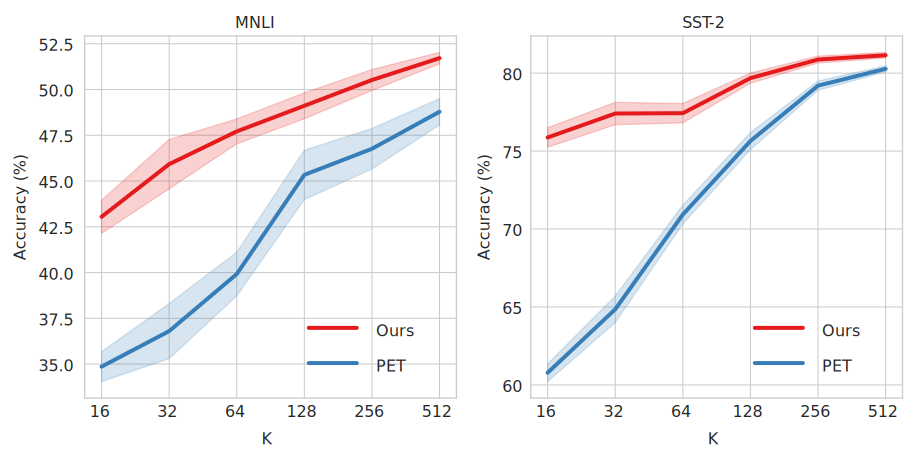
\includegraphics[width=0.7\textwidth]{plot.pdf}
	\bicaption{在不同训练样本规模 $K$ 下,Prompt-Distiller 与无蒸馏学生模型在 SST-2 和 MNLI 上的性能对比。随着 $K$ 增大,两者差距逐渐缩小,但 Prompt-Distiller 始终保持优势。}{Performance comparison between Prompt-Distiller and a student model trained without distillation under varying training set sizes $K$, illustrated on SST-2 and MNLI. As $K$ increases, the performance gap narrows, yet Prompt-Distiller consistently outperforms the baseline.}
	\label{fig:datasize}
\end{figure}

\mysubsubsection{不同学生模型规模分析}

接下来,我们将学生模型从默认的BERT-small换成BERT-base和BERT-tiny,来验证Prompt-Distiller对于更大或更小学生模型的适用性。表\ref{tab:model-scale}列出了SST-2、MPQA、MNLI上三种学生模型的蒸馏前后性能。可以看到:

对于BERT-base学生模型(参数1.1亿,接近教师模型的1/3),其不蒸馏时的few-shot提示微调准确率在三任务上分别为66.1\%、67.2\%、40.4\%,远高于BERT-small的下界(这符合直觉:模型大一些则容易拟合少量数据)。经过Prompt-Distiller蒸馏后,BERT-base性能进一步提升到87.8\%、84.0\%、51.5\%,几乎已追平教师模型在MNLI上的水平(51.5\% vs 教师FT 52\%左右)并超越教师模型在SST-2、MPQA上的上界。这说明Prompt-Distiller同样能使较大容量的学生模型受益,其学习到的教师知识足以弥补BERT-base与RoBERTa-large结构差异带来的性能落差。
对于极小的BERT-tiny模型(参数1500万,仅教师的4.2\%),不蒸馏时表现较差(SST-2仅56.8\%,MNLI仅33.6\%),几乎不能胜任复杂任务。蒸馏后,它们分别提高到62.4\%、34.8\%,虽然绝对增幅有限,但方向依然是积极的。在MNLI上BERT-tiny蒸馏只提高了1.2个百分点,因为模型容量实在过小,难以承载大量知识。但在SST-2上提升了5.6个百分点,说明即使极小模型,Prompt-Distiller也能赋予其一定的进步空间。实际上,对于BERT-tiny这样容量的模型,更适合用于简单任务或作为特定系统模块,但从实验可知本章方法对其仍有作用。
对于默认的BERT-small,我们之前已经详述,蒸馏效果最佳,平均涨幅9个百分点以上。

综合而言,Prompt-Distiller适用于不同尺寸的学生模型:对于容量较大的学生(如base),蒸馏使其如虎添翼,在few-shot下达到甚至超过教师的水平;对于极小模型,蒸馏虽受限于容量,收益较小但仍有提升;对于中等小模型,收益最显著。这说明双教师和对比学习策略并非针对某一特定规模模型,而是一种普适的知识迁移增强手段。

\begin{table}[htbp]
	\centering
	\bicaption[不同学生模型容量对比]{不同学生模型容量下Prompt-Distiller的蒸馏效果比较。每格中“$A/B$”分别表示不蒸馏时学生模型准确率$A$及蒸馏后的准确率$B$(\%)。}[Student model capacity comparison]{Comparison of Prompt-Distiller's distillation effects under different student model capacities. Each cell “$A/B$” reports the student accuracy without distillation ($A$) and after distillation ($B$) in \%.}
	\label{tab:model-scale}
	\small\begin{tabular}{l|ccc}
		\toprule[1pt]
		\textbf{学生模型}       & \textbf{SST-2} & \textbf{MPQA} & \textbf{MNLI} \\
		\midrule[0.5pt]
		BERT-base (12层110M) & 66.1 / 87.8    & 67.2 / 84.0   & 40.4 / 51.5   \\
		BERT-small (4层29M)  & 62.5 / 78.4    & 63.9 / 75.5   & 34.8 / 43.3   \\
		BERT-tiny (2层15M)   & 56.8 / 62.4    & 60.6 / 67.1   & 33.6 / 34.8   \\
		\bottomrule[1pt]
	\end{tabular}
\end{table}

\mysubsection{案例研究}
\label{sec:ch3-5-5-case-study}
最后,我们通过一个具体案例直观展示Prompt-Distiller如何融合双教师知识来提升学生模型的输出能力。表\ref{tab:case-study}列出了在SST-2情感分析任务上,一个测试样本经不同模型处理后的[MASK]预测结果。该样本是一个影评句对:\textit{“it all adds up to good fun. it was [MASK].”}(大意:“这一切加在一起很好玩。这部电影真是[MASK]。”)正确的情感标签是正面,对应的标签词我们选取great。

\begin{table}[htbp]
	\centering
	\bicaption{影评句“it was [MASK].”在不同模型下输出概率最高的几个词。可以看出,提示微调教师和预训练教师都将积极色彩的great列为高概率预测词,而学生模型经Prompt-Distiller蒸馏后也成功地将great作为最高概率词输出。}{The phrase “it was [MASK]” in film reviews yields several words with the highest output probabilities across different models. It is evident that both the prompt-fine-tuned teacher and the pre-trained teacher list the positive-toned ‘great’ as a high-probability prediction. Similarly, after undergoing Prompt-Distiller distillation, the student model also successfully outputs great as the word with the highest probability.}
	\label{tab:case-study}
	\small\begin{tabular}{l|p{6cm}}
		\toprule[1pt]
		\textbf{模型}                   & \multicolumn{1}{c}{\textbf{Top-3候选词}}       \\
		\midrule[0.5pt]
		提示微调教师 RoBERTa-large          & \texttt{\small great, brilliant, good, ...} \\
		原始预训练教师 RoBERTa-large         & \texttt{\small fun, great, good, ...}       \\
		Prompt-Distiller学生 BERT-small & \texttt{\small great, shaken, ...}          \\
		\bottomrule[1pt]
	\end{tabular}
\end{table}

从表\ref{tab:case-study}可以看到:提示微调后的RoBERTa-large教师模型在该提示`it was [MASK].''处的预测中,把表示棒极了的词great排在第一位,紧随其后的是“brilliant”(精彩的)、good(好的)等正面词汇。原始未微调的RoBERTa-large预训练模型虽然不知道当前任务是情感分类,但由于庞大的语料记忆,它在`it was [MASK].''后最有可能填入的词也是带有积极含义的fun(有趣)、great、good等。这说明预训练模型本身具有一定的常识:当一句话说“很好玩,这真是\_\_\_”,大概率是正面评价。学生模型BERT-small在未经蒸馏前,很可能无法正确预测这个[MASK]词(我们观察到未蒸馏学生往往给出无关或中性词)。但经过Prompt-Distiller训练后,学生模型的最高概率预测词同样变成了great,第二高为shaken(这里是干扰项,可能由于学生容量小出现),其他备选也更贴近正面倾向。这个例子生动地表明:通过Prompt-Distiller,学生模型成功地从提示微调教师那里学到了任务相关的倾向(即选择正面词汇),也从预训练教师那里继承了对常见表达的判断(如将great视为高度相关的填空)。两方面知识的融合,使学生模型给出了正确的输出,并且较好地模拟了大模型的行为。这与我们设计Prompt-Distiller的初衷一致,即学生模型不仅在硬指标上逼近教师,在行为上也越来越像教师,对任务的理解更加全面准确。

\mysection{本章小结}
\label{sec:ch3-6-chapter-summary}
本章围绕少样本提示学习模型的压缩问题,提出了Prompt-Distiller算法,并通过理论推导和实验证明了其有效性。我们以预训练语言模型的提示微调为背景,引入双教师机制和探针对比学习,实现了在极少标注数据条件下的小模型高效蒸馏。通过来自提示微调教师的任务特定知识和来自预训练教师的通用知识相结合,学生模型克服了训练数据匮乏的限制;而基于对比学习的中间层知识迁移则进一步提升了学生对教师深层判别模式的掌握。从多个任务的实验结果看,Prompt-Distiller显著提高了学生模型的精度,在一些任务上甚至达到或超过教师模型的表现,充分验证了多层次知识迁移策略的作用。同时,我们分析了各组件的贡献,发现无标注数据提供的预训练知识是提升关键,而探针对比学习亦增强了蒸馏效果;数据规模和模型规模实验则展示了Prompt-Distiller的通用适用性。最后通过案例直观说明了学生模型如何通过蒸馏变得更聪明。

本章的研究为小样本条件下深度模型的高效构建提供了新的思路,即利用大模型蕴含的不同层次知识指导小模型训练,从而弥补后者在数据和容量上的不足。这种方法与前章提出的多层次知识迁移框架一脉相承,证明了多层次知识在模型压缩领域的价值。本章的研究结果为下一章的系统实现提供了理论依据:我们将在下一章探讨如何将Prompt-Distiller蒸馏得到的小模型应用于实际的在线服务系统,并结合其他优化手段,实现深度模型在工业场景下的高效部署与推理。

\end{document}
